\section{Componentes principales de un sistema operativo}

Un sistema operativo integra diversos componentes que gestionan los recursos de hardware y ofrecen servicios a los procesos que se ejecutan en el sistema.  

\subsection{Gestión de procesos}

La gestión de procesos es uno de los pilares fundamentales de cualquier sistema operativo, ya que se encarga de controlar la ejecución de programas y de garantizar un uso eficiente de la CPU. Un proceso, desde su creación hasta su finalización, pasa por diferentes estados a lo largo de su ciclo de vida. Al crearse, entra en el estado nuevo; luego pasa al estado preparado mientras espera acceso a la CPU. Cuando el planificador lo selecciona, pasa a ejecutando. Durante la ejecución, un proceso puede quedar en espera si requiere operaciones de entrada/salida, y finalmente alcanza el estado terminado al completar su tarea, como se muestra en la Figura \ref{fig:ciclo_vida_proceso}.  

\begin{figure}[H]
    \centering
    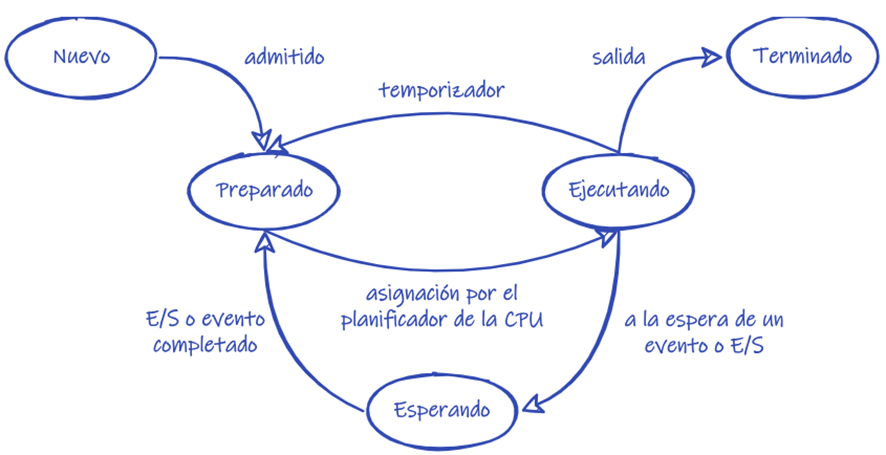
\includegraphics[width=0.7\textwidth]{figures/ciclo_vida_proceso.png}
    \caption[Diagrama de estados de un proceso]%
            {Diagrama de estados de un proceso. Fuente: \citep{torres2024}}
    \label{fig:ciclo_vida_proceso}
\end{figure}

Entre las funciones principales de la gestión de procesos se encuentra la creación y finalización de procesos. El sistema operativo se encarga de iniciar nuevos procesos mediante llamadas al sistema (por ejemplo, \texttt{fork} en Unix) y de eliminar aquellos que ya han concluido su ejecución \citep{juan2015}.  

Otra función esencial es la planificación o \textit{scheduling}, que consiste en decidir el orden en el que los procesos acceden a la CPU. Para ello se emplean algoritmos como FIFO, round robin o planificación basada en prioridades, según los objetivos de rendimiento y equidad del sistema \citep{juan2015}.  

Asimismo, la gestión de procesos incluye mecanismos de sincronización y comunicación, conocidos como IPC (Inter-Process Communication). Estos permiten que los procesos se coordinen y compartan información de manera segura, evitando condiciones de carrera y conflictos al acceder a recursos comunes \citep{wikipedia}.  
\newpage
\begin{muntab}{|p{4cm}|p{9cm}|}
  {razones_creacion_procesos}
  {Razones comunes para la creación de procesos en un sistema operativo \citep{sistemas_operativos}}
\hline
\textbf{Tipo de proceso} & \textbf{Descripción} \\
\hline
Proceso por lotes & El SO procesa trabajos en lote desde cinta/disco. Lee secuencias de control de trabajos automáticamente. \\
\hline
Sesión interactiva & Usuario inicia sesión desde un terminal. \\
\hline
Servicio del sistema & El SO crea procesos para servicios en segundo plano (ej: impresión) sin espera del usuario. \\
\hline
Proceso hijo & Proceso existente crea nuevos procesos para modularidad o paralelismo. \\
\hline
\end{muntab}
\newpage
\begin{muntab}{|p{4cm}|p{10cm}|}
  {razones_terminacion}
  {Razones comunes para la terminación de procesos en un sistema operativo \citep{sistemas_operativos}}
\hline
\textbf{Causa de terminación} & \textbf{Descripción} \\
\hline
Finalización normal & Completación voluntaria mediante llamada al sistema. \\
\hline
Límite de tiempo & Exceso de tiempo de ejecución o espera. \\
\hline
Memoria no disponible & Memoria insuficiente o acceso no permitido. \\
\hline
Error de protección & Uso no autorizado de recursos. \\
\hline
Error aritmético & Operación inválida (ej: división por cero). \\
\hline
Fallo de E/S & Error en operación de entrada/salida. \\
\hline
Instrucción inválida & Ejecución de instrucción inexistente. \\
\hline
Instrucción privilegiada & Uso de instrucción reservada al SO. \\
\hline
Datos inapropiados & Datos erróneos o no inicializados. \\
\hline
Intervención externa & Terminación por operador o SO. \\
\hline
Terminación por padre & Finalización por proceso padre (automática o solicitada). \\
\hline
\end{muntab}
\newpage
\subsection{Gestión de memoria}

La gestión de memoria es esencial para que el sistema operativo asigne y libere espacio en la memoria principal (RAM) a los procesos en ejecución. Su función principal consiste en aislar los espacios de direcciones de cada programa, de modo que puedan ejecutarse de manera concurrente sin interferir entre sí. Gracias a este control, la CPU puede cargar en memoria las instrucciones y datos necesarios de cada proceso en el momento oportuno. En términos generales, el administrador de memoria organiza los procesos de tal manera que se obtenga la máxima utilidad del espacio disponible, trasladando a la memoria principal la información que debe ejecutarse en cada instante \citep{wikipedia1}.  

En los sistemas modernos esta gestión se fundamenta en el concepto de memoria virtual, que proporciona a cada proceso una memoria lógica mayor que la memoria física disponible. Para ello se emplean técnicas como la paginación, en las que cada proceso dispone de su propia tabla de páginas que mapea direcciones lógicas hacia marcos de la memoria física. En la Figura \ref{fig:memoria} se ilustra este esquema, donde las páginas virtuales de los procesos se corresponden con bloques de memoria física compartida de manera ordenada.  

\begin{figure}[H]
    \centering
    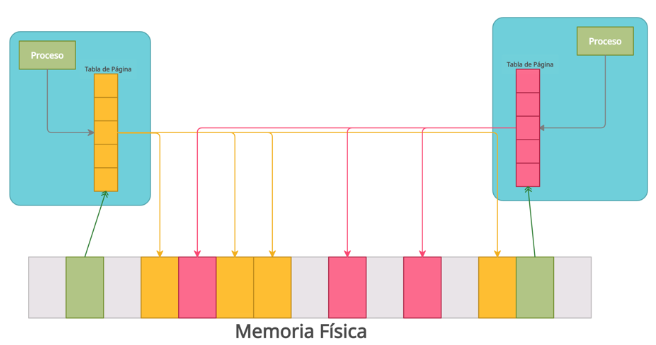
\includegraphics[width=0.8\textwidth]{figures/memoria.png}
    \caption{Traducción por paginación. Cada proceso (cajas turquesa) posee su propia tabla de páginas (columnas amarilla y rosada) que asigna páginas lógicas a marcos de la memoria física (bloques coloreados). Fuente: \citep{wikipedia2}}
    \label{fig:memoria}
\end{figure}

Entre las funciones principales del gestor de memoria se encuentran el control del uso de la memoria, la asignación y liberación de espacio para los procesos, la reubicación de datos en caso necesario, la gestión de la fragmentación y la compactación, la implementación de la memoria virtual y la protección de los espacios de direcciones para evitar accesos indebidos entre procesos. Estas tareas en conjunto garantizan un uso eficiente y seguro del recurso más limitado y compartido del sistema.  

La traducción mediante paginación, como se aprecia en la figura, permite que cada proceso perciba su espacio de direcciones como contiguo, aunque en la práctica las páginas estén distribuidas en diferentes marcos físicos de la RAM. El sistema operativo se encarga de mantener actualizadas las tablas de páginas y, cuando es necesario, puede intercambiar páginas entre la memoria principal y el disco, asegurando así la abstracción de una memoria virtual continua \citep{ucm2020}.  
\subsection{Sistema de archivos}

\subsubsection{Estructura jerárquica}
El sistema de archivos organiza los archivos y directorios en forma de árbol invertido. A nivel lógico existe un único directorio raíz (/), 
nodo principal que contiene todos los demás. Cada nodo del árbol corresponde a un directorio que puede contener subdirectorios, archivos normales o especiales.
Este diseño jerárquico con nombres únicos por directorio facilita la navegación y la gestión, evitando colisiones de nombres.

\subsubsection{Gestión de datos persistentes}
El sistema de archivos provee los medios para almacenar y recuperar datos de forma ordenada en la memoria secundaria (discos, SSD, etc.). 
La memoria se divide en bloques de tamaño fijo, y el sistema de archivos asigna a cada archivo los bloques necesarios. 
Además, controla la consistencia de los datos mediante técnicas como journaling, asegurando que la información persista aunque finalicen los procesos o falle el sistema. 
También gestiona la integridad ante fallos, permitiendo recuperar estructuras de disco sin pérdida de datos~\citep{ual2019}.

\subsubsection{Operaciones de archivo}
El sistema de archivos ofrece llamadas básicas para crear, abrir, leer, escribir, renombrar y eliminar archivos y directorios. 
Por ejemplo, al invocar \texttt{open}, el kernel devuelve un descriptor de archivo que apunta a una entrada en la tabla de archivos abiertos y al inodo correspondiente. 
Según Bach (1986), esta tabla relaciona descriptores, entradas de acceso y estructuras de inodos internos. 
En otras palabras, cada proceso maneja un descriptor representado como un entero, mientras que el sistema mantiene internamente una tabla que referencia los inodos de los archivos abiertos~\citep{ual2019}.

\subsubsection{Asignación de espacio}
Los datos de cada archivo se almacenan en bloques de disco. El sistema de archivos controla qué bloques están libres y asigna los necesarios a cada archivo. 
En el esquema FAT (File Allocation Table), por ejemplo, cada disco dispone de una tabla con una entrada por bloque; cada entrada indica el siguiente bloque del archivo o un marcador especial que puede señalar bloque libre, bloque defectuoso o fin de archivo.

\subsubsection{Seguridad y atributos}
El sistema de archivos gestiona los atributos (metadatos) de cada archivo, así como la aplicación de permisos. 
En sistemas Unix, cada archivo se describe mediante un inodo que almacena permisos de acceso, propietario (UID/GID), fechas de modificación y tipo de archivo~\citep{ual2005}.
\subsubsection{Journaling}
El journaling es un mecanismo que permite implementar transacciones en los sistemas de archivos. 
También se conoce como registro por diario, ya que mantiene un journal donde se almacena la información necesaria para restablecer los datos afectados en caso de fallo. 
Por ejemplo, ante un corte de energía, al reiniciar se reproduce el journal para completar o deshacer operaciones, restaurando así la consistencia. 
Gracias a este enfoque, los sistemas de archivos pueden volver rápidamente a producción con menor riesgo de corrupción~\citep{wikipedia3}.

\subsection{Gestión de dispositivos (E/S)}
El sistema de entrada y salida del sistema operativo funciona como interfaz entre el hardware de los dispositivos (discos, teclados, impresoras, etc.) y el software, 
ocultando las particularidades de cada dispositivo al resto del sistema~\citep{torres2024}.  

Sus componentes principales son:
\begin{itemize}
    \item Controladores de dispositivo (drivers). Son programas específicos, normalmente provistos por el fabricante, que conocen los detalles del hardware y traducen las peticiones genéricas del sistema operativo en operaciones concretas sobre el dispositivo~\citep{torres2024}.
    \item Interfaz genérica de E/S. El sistema operativo ofrece llamadas estándar como \texttt{open}, \texttt{read}, \texttt{write}, \texttt{close} o \texttt{ioctl}, 
    de modo que los programas interactúan con los dispositivos sin necesidad de conocer sus características físicas. 
    En sistemas UNIX, todos los dispositivos de E/S se representan como archivos dentro del directorio \texttt{/dev}, lo que permite operaciones uniformes~\citep{torres2024}.
    \item Buffering y caching. El buffering compensa diferencias de velocidad durante transferencias de datos en curso, mientras que el caching se centra en la reutilización de datos accedidos recientemente, anticipando futuras solicitudes para acelerar accesos posteriores.
    \item Spooling. En dispositivos secuenciales no compartibles, como impresoras, el sistema operativo encola los trabajos de varios procesos en un almacenamiento intermedio, 
    gestionándolos en orden sin bloquear a los procesos que los enviaron~\citep{torres2024}.
\end{itemize}

En conjunto, la gestión de dispositivos permite a los procesos leer y escribir en hardware diverso mediante una interfaz uniforme, mientras el sistema operativo optimiza el flujo de datos y protege el acceso concurrente.

\subsection{Interfaz de usuario}
La interfaz de usuario es el medio a través del cual las personas interactúan con el sistema operativo.
\begin{figure}[H]
    \centering
    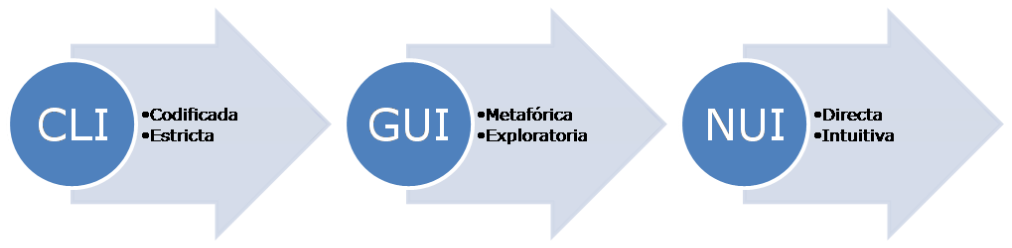
\includegraphics[width=0.7\textwidth]{figures/interfaz.png}
    \caption[Evolución de las interfaces de usuario]%
            {Evolución de las interfaces de usuario \citep{wikipedia4}}
    \label{fig:Evolucion_Interfaz}
\end{figure}

Las interfaces de usuario han evolucionado en diferentes formas de interacción:
\begin{itemize}
    \item CLI (Command Line Interface). El usuario escribe comandos en una consola o terminal.
    \item GUI (Graphical User Interface). Interfaz gráfica con ventanas, iconos y menús, más intuitiva y exploratoria.
    \item NUI (Natural User Interface). Interacción más directa e intuitiva, basada en mecanismos como el tacto, la voz o los gestos.
\end{itemize}

Un buen diseño de interfaz busca usabilidad e intuición, permitiendo al usuario dar órdenes al sistema operativo y visualizar información de estado. 
Esto incluye terminales, escritorios, menús de configuración o iconos de carpeta. El estilo de interfaz puede variar mucho entre sistemas, 
desde texto puro en algunos Unix básicos hasta entornos gráficos completos en sistemas modernos.

\subsection{Seguridad y protección}
La seguridad en un sistema operativo busca garantizar que solo los usuarios autorizados utilicen los recursos y lo hagan de la manera adecuada. 
Uno de los principios fundamentales es el de menor privilegio: cada proceso recibe únicamente los permisos estrictamente necesarios.  
La autenticación permite identificar al usuario, generalmente mediante contraseña, y asignar permisos correspondientes. 
En sistemas como Multics, un servicio de autenticación asocia cada proceso a un usuario; si este servicio falla, un proceso podría recibir permisos indebidos al quedar vinculado con un usuario equivocado~\citep{columbia2008}.

\subsubsection{Control de acceso}
El sistema operativo aplica un modelo de control de acceso que asigna permisos a los distintos recursos (archivos, dispositivos, regiones de memoria, etc.).  
Cada solicitud de un proceso se comprueba mediante un monitor de referencia, que valida las operaciones de acuerdo con los permisos asignados.  
De manera conceptual, esta verificación puede representarse como una matriz de acceso, donde las filas corresponden a procesos o dominios, 
las columnas a objetos del sistema y las celdas a los permisos de lectura, escritura o ejecución.  

En Unix, por ejemplo, cada archivo tiene bits de permiso y un propietario, siendo este último quien puede modificar los bits de acceso del archivo~\citep{columbia2008}.
\subsubsection{Aislamiento de procesos y protección de memoria}
El sistema operativo protege la memoria y el contexto de cada proceso para impedir interferencias entre ellos. Cada proceso se ejecuta en modo usuario (no privilegiado) dentro de su propio espacio virtual de direcciones.  
De esta manera, ningún proceso puede leer o escribir directamente en la memoria de otro, ni en la memoria del núcleo.  
La protección de memoria asegura que los datos de un usuario no puedan ser accedidos por otro y que el código crítico del kernel permanezca intacto.  

Un ejemplo de este mecanismo es la arquitectura de privilegios o *rings*, donde las instrucciones sensibles solo se permiten en modo kernel (nivel 0).  
En este nivel privilegiado se ejecutan las operaciones críticas sobre memoria y dispositivos~\citep{princeton2018}.

\subsubsection{Prevención de intrusiones}
Además de la protección interna, el sistema operativo incorpora mecanismos activos frente a amenazas externas o internas.  
Un sistema de prevención de intrusiones (IPS) supervisa el tráfico y la actividad en busca de comportamientos anómalos, ya sea mediante firmas conocidas o por detección de desviaciones.  
Si se identifica una amenaza, el IPS puede bloquearla antes de que cause daño, por ejemplo cerrando conexiones peligrosas o eliminando contenido malicioso.  

Estos mecanismos suelen incluir filtros y cortafuegos integrados en el sistema operativo, que rechazan accesos no autorizados —ya sea por red o de manera local— según las políticas definidas.  
En conjunto, el sistema previene ataques como virus, intrusiones de red o escaladas de privilegios, al analizar cada petición de acceso y denegarla cuando coincide con patrones maliciosos~\citep{ibm2019}.

\subsubsection{Auditoría y registro}
Con el fin de detectar incidentes y comportamientos sospechosos, el sistema operativo mantiene registros de auditoría de eventos relevantes: inicios y cierres de sesión, errores de autenticación, intentos fallidos de acceso, cambios en permisos, entre otros.  
Cada evento se almacena con la fecha, el usuario y la acción realizada, lo que permite revisar los logs para identificar accesos indebidos o intrusiones después de que ocurran.  

Los sistemas de auditoría más avanzados incluso generan alertas automáticas al equipo de seguridad cuando detectan anomalías en el comportamiento~\citep{ibm2019}.

\subsubsection{Modelos de seguridad clásicos}
En sistemas operativos con seguridad reforzada también se emplean modelos formales que definen con rigor las reglas de acceso.  
El modelo Bell–LaPadula se centra en la confidencialidad, aplicando el principio de “no leer hacia arriba, no escribir hacia abajo” (*read down, write up*).  
Con ello, un sujeto solo puede leer información de igual o menor nivel de clasificación y escribir en niveles iguales o superiores, evitando fugas de datos sensibles.  

Por otro lado, el modelo Biba protege la integridad mediante las reglas opuestas: “read up, write down”.  
Así se evita que un proceso de baja integridad contamine a uno de mayor integridad, o que datos críticos se vean corrompidos por información poco confiable.  

En la práctica, estos modelos, junto con variantes como Clark–Wilson, proporcionan una base sólida para garantizar tanto la confidencialidad como la integridad en sistemas multigrado~\citep{columbia2008}.

